\documentclass[letterpaper,12pt,fleqn]{article}
\usepackage{matharticle}
\pagestyle{empty}
\newcommand{\norm}[1]{\left\|#1\right\|}
\renewcommand{\mp}{\mathcal{P}}
\newcommand{\mc}{\mathcal{C}}
\renewcommand{\a}{\alpha}
\renewcommand{\b}{\beta}
\renewcommand{\l}{\lambda}
\newcommand{\e}{\epsilon}
\newcommand{\vx}{\vec{x}}
\begin{document}
\section*{Banach Spaces}

\begin{definition}[Banach]
  Let $E$ be a normed space. To say that $E$ is \emph{complete} means that
  every Cauchy sequence in $E$ converges to some element of $E$.

  A complete normed space is called a \emph{Banach} space.
\end{definition}

\begin{examples}
  \listbreak
  \begin{enumerate}
  \item $E=\mp[a,b]$ with the sup (uniform convergence) norm is not Banach.

    As a counterexample, consider $f_n=\sum_{k=1}^n\frac{t^k}{k!}\in\mp[0,1]$

    AWLOG: $n<m$.
    
    $\norm{f_n-f_m}=
    \norm{\sum_{k=1}^m\frac{t^k}{k!}-\sum_{k=1}^n\frac{t^k}{k!}}=
    \norm{\sum_{k=n+1}^m\frac{t^k}{k!}}=
    \sum_{k=n+1}^m\frac{1}{k!}\to0$

    Thus, $f_n$ is Cauchy; however, $f_n\to f=e^t\notin\mp[0,1]$.

    Therefore, $\mp[0,1]$ is not Banach.

  \item $E=\mc[0,1]$ with $\norm{f}=\int_0^1\abs{f(t)}dt$ is not Banach.

    As a counterexample, consider $f_n=t^n\in\mc[0,1]$.

    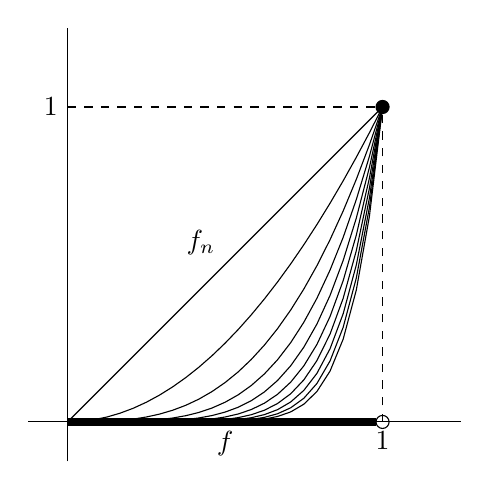
\begin{tikzpicture}
      \draw (-0.5,0) -- (5,0);
      \draw (0,-0.5) -- (0,5);
      \node [below] at (4,0) {$1$};
      \node [left] at (0,4) {$1$};
      \draw [dashed] (0,4) -- (4,4);
      \draw [dashed] (4,0) -- (4,4);
      \draw [domain=0:4] plot ({\x},{\x});
      \draw [domain=0:4] plot ({\x},{4*(\x/4)^2});
      \draw [domain=0:4] plot ({\x},{4*(\x/4)^3});
      \draw [domain=0:4] plot ({\x},{4*(\x/4)^4});
      \draw [domain=0:4] plot ({\x},{4*(\x/4)^5});
      \draw [domain=0:4] plot ({\x},{4*(\x/4)^6});
      \draw [domain=0:4] plot ({\x},{4*(\x/4)^7});
      \draw [domain=0:4] plot ({\x},{4*(\x/4)^8});
      \draw [domain=0:4] plot ({\x},{4*(\x/4)^9});
      \draw [domain=0:4] plot ({\x},{4*(\x/4)^10});
      \node [draw, circle, scale=0.5] (a) at (4,0) {};
      \node [draw, fill, circle, scale=0.5] (b) at (4,4) {};
      \draw [line width=1mm] (0,0) to (a);
      \node [above left] at (2,2) {$f_n$};
      \node [below] at (2,0) {$f$};
    \end{tikzpicture}

    Claim: $f_n$ is Cauchy in the norm.

    AWLOG: $n<m$
    
    \begin{eqnarray*}
      \norm{f_n-f_m} &=& \int_0^1\abs{f_n-f_m} \\
      &=& \int_0^1(t^n-t^m)dt \\
      &=& \left[\frac{1}{n+1}t^{n+1}-\frac{1}{m+1}t^{m+1}\right]_0^1 \\
      &=& \frac{1}{n+1}-\frac{1}{m+1} \\
      &\to& 0
    \end{eqnarray*}

    Claim: $f_n\to f$ where
    $f=\begin{cases}0, & 0\le x<1 \\ 1, & x=1\end{cases}$

    \begin{eqnarray*}
      \norm{f_n-f} &=& \norm{f_n-0} \\
      &=& \norm{f_n} \\
      &=& \int_0^1t^ndt \\
      &=& \left.\frac{1}{n+1}t^{n+1}\right|_0^1 \\
      &=& \frac{1}{n+1} \\
      &\to& 0
    \end{eqnarray*}

    Thus, $f_n$ is Cauchy in the norm and $f_n\to f$ in the norm; however, $f$
    is discontinuous and thus $f\notin\mc[0,1]$.

    Therefore, $\mc[0,1]$ is not complete, and thus not Banach.

  \item $E=\mc[a,b]$ with the sup (uniform convergence) norm is Banach.

    Assume $(f_n)$ in $\mc[a,b]$ is Cauchy. \\
    Thus, $\forall\,\e>0,\exists\,N>0,n,m>N\implies\norm{f_n-f_m}<\e$.

    $\abs{f_n(x)-f_m(x)}\le\max_{x\in[a,b]}\abs{f_n-f_m}=\norm{f_n-f_m}<\e$

    Thus, $\forall\,x\in[a,b],(f_n(x))$ is Cauchy. \\
    So by completeness of $\R$, $\forall\,x\in[a,b],f_n(x)\to f(x)$. \\
    By letting $m\to\infty$, $\forall\,x\in[a,b],\abs{f_n(x)-f(x)}<\e$. \\
    Thus, $f_n\rightrightarrows f$ and is $f_n$ continuous, so $f$ is also
    continuous and $f\in\mc[a,b]$.

    Therefore, $\mc[a,b]$ is Banach.

  \item $\ell^p$ with
    $\norm{x}_p=\left(\sum_{k=1}^{\infty}(x_n)^p\right)^{\frac{1}{p}}$ is Banach
    for $1\le p<\infty$.

    Assume $(\a_n)$ is a Cauchy sequence (of sequences) in $\ell^p$, where
    $\a_n=(\a_{n,1},\a_{n,2},\ldots)$. \\
    Assume $\e>0$.
    \[\exists\,N>0,n,m>N\implies\norm{\a_n-\a_m}=
    \left(\sum_{k=1}^{\infty}\abs{\a_{n,k}-\a_{m,k}}^p\right)^{\frac{1}{p}}<\e\]
    And so:
    \[\sum_{k=1}^{\infty}\abs{\a_{n,k}-\a_{m,k}}^p<\e^p\]
    Thus, for each fixed $k$:
    \[\abs{\a_{n,k}-\a_{m,k}}^p\le\sum_{k=1}^{\infty}\abs{\a_{n,k}-\a_{m,k}}^p<
    \e^p\]
    And so:
    \[\abs{\a_{n,k}-\a_{m,k}}<\e\]
    Thus, for each fixed $k$, the sequence $(\a_{n,k})$ is Cauchy in $\C$. \\
    But $\C$ is complete, so $\a_{n,k}\to\a_k\in\C$. \\
    Let $\a=(\a_n)$, i.e., $\a$ is the sequence of the limits.

    By letting $m\to\infty$ and assuming $n>N$:
    \[\sum_{k=1}^{\infty}\abs{\a_{n,k}-\a_k}^p<\e^p<\infty\]
    Furthermore, since $\a_N\in\ell^p$:
    \[\sum_{k=1}^{\infty}\abs{\a_N,k}^p<\infty\]
    Now, applying Minkowski:
    \begin{eqnarray*}
      \left(\sum_{k=1}^{\infty}\abs{\a_k}^p\right)^{\frac{1}{p}} &=&
      \left(\sum_{k=1}^{\infty}[(\abs{\a_k}-\abs{\a_{N,k}})+\abs{\a_{N,k}}]^p
      \right)^{\frac{1}{p}} \\
      &\le& \left(\sum_{k=1}^{\infty}(\abs{\a_k}-\abs{\a_{N,k}})^p
      \right)^{\frac{1}{p}}+
      \left(\sum_{k=1}^{\infty}\abs{\a_{N,k}}^p\right)^{\frac{1}{p}} \\
      &\le& \left(\sum_{k=1}^{\infty}\abs{\a_k-\a_{N,k}}^p\right)^{\frac{1}{p}}+
      \left(\sum_{k=1}^{\infty}\abs{\a_{N,k}}^p\right)^{\frac{1}{p}} \\
      &<& \infty
    \end{eqnarray*}
    Therefore, $\a\in\ell^p$.

    Moreover:
    \[\norm{\a_n-\a}=\left(\sum_{k=1}^{\infty}\abs{\a_{n,k}-\a_k}^p
    \right)^{\frac{1}{p}}<\e\]
    And so $\norm{\a_n-\a}\to0$.

    Thus, $\a_n\to\a\in\ell^p$, so $\ell^p$ is complete and therefore Banach.

  \item $\ell^{\infty}$ with $\norm{x}_{\infty}=\sup_{n\in\N}\abs{x_n}$ is
    Banach.

    Assume $(\a_n)$ is a Cauchy sequence (of sequences) in $\ell^{\infty}$,
    where $\a_n=(\a_{n,1},\a_{n,2},\ldots)$. \\
    Assume $\e>0$.
    \[\exists\,N>0,n,m>N\implies\norm{\a_n-\a_m}=
    \sup_{k\in\N}\abs{\a_{n,k}-\a_{m,k}}<\e\]
    And so:
    \[\abs{\a_{n,k}-\a_{m,k}}\le\sup_{k\in\N}\abs{\a_{n,k}-\a_{m,k}}<\e\]
    Thus, for each fixed $k$, the sequence $(\a_{n,k})$ is Cauchy in $\C$. \\
    But $\C$ is complete, so $\a_{n,k}\to\a_k\in\C$. \\
    Let $\a=(\a_n)$, i.e., $\a$ is the sequence of the limits.

    By letting $m\to\infty$ and assuming $n>N$:
    \[\sup_{k\in\N}\abs{\a_{n,k}-\a_k}<\e<\infty\]
    Furthermore, since $\a_N\in\ell^{\infty}$:
    \[\sup_{k\in\N}\abs{\a_N,k}<\infty\]
    Now, to show that $\a\in\ell^{\infty}$:
    \begin{eqnarray*}
      \sup_{k\in\N}\abs{\a_k} &=&
      \sup_{k\in\N}\{(\abs{\a_k}-\abs{\a_{N,k}})+\abs{\a_{N,k}}\} \\
      &\le& \sup_{k\in\N}\{\abs{\a_k}-\abs{\a_{N,k}}\}+
      \sup_{k\in\N}\abs{\a_{N,k}} \\
      &<& \infty
    \end{eqnarray*}
    Therefore, $\a\in\ell^{\infty}$.

    Moreover:
    \[\norm{\a_n-\a}=\sup_{k\in\N}\abs{\a_{n,k}-\a_k}<\e\]
    And so $\norm{\a_n-\a}\to0$.

    Thus, $\a_n\to\a\in\ell^{\infty}$, so $\ell^{\infty}$ is complete and
    therefore Banach.
  \end{enumerate}
\end{examples}

\begin{theorem}
  Let $E$ be a Banach space and $F$ a closed subspace of $E$. $F$ is also
  Banach.
\end{theorem}

\begin{theproof}
  Assume $(\vx_n)$ is Cauchy in $F$. \\
  Thus $(\vx_n)$ is Cauchy in $E$ and $\vx_n\to\vx\in E$, since $E$ is
  complete. \\
  But $F$ is closed and thus contains all of its limit points, and so
  $\vx\in F$.

  Therefore $F$ is complete, and thus Banach.
\end{theproof}

\end{document}
